\documentclass{article}
\usepackage{graphicx}
\usepackage{tocloft} 
\usepackage{glossaries}
\usepackage{lipsum}
\usepackage{geometry}
\usepackage{fancyhdr} 
\usepackage{amsmath}
\usepackage{biblatex}  
\geometry{a4paper, margin=1in}

\title{Design Specification}
\author{Group 1 }
\date{\today}

\begin{document}
\maketitle  
\pagebreak

\tableofcontents
\pagebreak


\includegraphics[width=0.3\linewidth]{../logo/csula.png} 
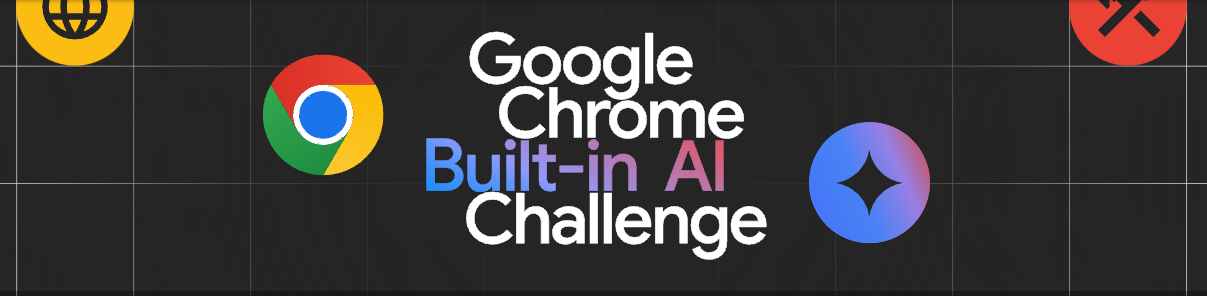
\includegraphics[width=0.3\linewidth]{../logo/chromeai.png}

\section{Introduction}
\subsection{Purpose}
This document outlines the system architecture, UI components, and data structures that were used for our Chrome AI-Enhanced Web Application. It should serve as a blueprint for developers, designers, and stakeholders to learn and understand the design decisions and underlying technologies for this product.

\subsection{Scope}
The specifications will cover the frontend (in this case the Chrome extension), the AI API integrations, and the backend components that go into this.

\section{System Architecture}
The application runs entirely in the browser, using Chrome’s built-in AI APIs. The way this works is as follows:
\begin{enumerate}
    \item User interacts with the UI elements in the Chrome Extension.
    \item UI sends a request to the AI APIs (Prompt, Summarization, Translation, Rewrite).
    \item The AI models process the input and then return the results.
    \item UI updates dynamically to display results without the need of any server calls.
\end{enumerate}

\section{Page-by-Page Breakdown}
\subsection{Main Dashboard}
\begin{itemize}
    \item \textbf{Purpose:} Central hub where all the AI features will be accessed from.
    \item \textbf{UI Elements:}
    \begin{itemize}
        \item Navigation bar with links to "Prompts", "Summarize", "Translate", "Rewrite".
        \item A responsive layout
    \end{itemize}
    \item \textbf{Data Flow:} User input in forms is sent to the relevant AI API and then processed. 
\end{itemize}

\subsection{Prompt Page}
\begin{itemize}
    \item \textbf{Purpose:} Generate dynamic prompts based on the user's queries.
    \item \textbf{UI Elements:} Text field for input, "Generate Prompt" button, and results area.
    \item \textbf{Interactions:} User clicks "Generate Prompt" → JS function sends input to Prompt API → Render the suggestion below.
\end{itemize}

\subsection{Summarize Page}
\begin{itemize}
    \item \textbf{Purpose:} Provide concise summaries of long texts.
    \item \textbf{UI Elements:} Large text area for input, upload option, "Summarize" button, and results panel.
    \item \textbf{Interactions:} Input text or selected file → Summarization API → Output a summarized version of the writing.
\end{itemize}

\subsection{Translate Page}
\begin{itemize}
    \item \textbf{Purpose:} Translate text between languages.
    \item \textbf{UI Elements:} Source text area, language selectors (dropdowns), and "Translate" button.
    \item \textbf{Interactions:} Input text + selected languages → Translation API → Output in target language area.
\end{itemize}

\subsection{Rewrite Page}
\begin{itemize}
    \item \textbf{Purpose:} Suggest alternative phrasings for user-provided text.
    \item \textbf{UI Elements:} Text input area, "Rewrite" button, suggestions panel.
    \item \textbf{Interactions:} User pastes text → Clicks "Rewrite" → API returns multiple suggestions → User selects a preferred suggestion.
\end{itemize}

\section{Components and Tools}
\subsection{Frontend Components}
\begin{itemize}
    \item \textbf{React.js}: A library particularly designed for web applications and UI.
    \item \textbf{Material UI}: A library that provides ready-made UI components and layout grids.
\end{itemize}

\subsection{AI APIs}
\begin{itemize}
    \item \textbf{Prompt API}: Accepts user queries, returns suggestions.
    \item \textbf{Summarization API}: Converts long text into a short summary.
    \item \textbf{Translation API}: Translates text between supported languages.
    \item \textbf{Rewrite API}: Suggests alternative wordings.
\end{itemize}

\section{Performance Considerations}
The AI APIs run locally, this was done in order to allow for quick responses and minimal latency.

\section{Accessibility}
\begin{itemize}
    \item Option to customize font size.
    \item Light and Dark mode.
    \item Multiple languages.
    \item Proper ARIA labels for screen reader support.
\end{itemize}

\section{Future Enhancements}
\begin{itemize}
    \item There are plants to add voice commands in order to allow for hands-free operations.
    \item The translation is limited to the languages provided by the API so there are plans of adding even more languages.
\end{itemize}

\end{document}
